\documentclass[10pt]{beamer}
\usepackage[english]{babel}
\usepackage[utf8]{inputenc}
\usepackage[T1]{fontenc}
\usepackage{helvet}

%-------------------------------------------------------
% INFORMATION IN THE TITLE PAGE
%-------------------------------------------------------

\newcommand{\cstitle}{\textbf{Bioinformatics}}
\subtitle[]{Genome by numbers}
\newcommand{\cscourseCode}{1005155}
\newcommand{\csauthor}{MSc. Vicente Machaca Arceda}
\institute[UNSA]{Universidad Nacional de San Agustín de Arequipa}
\newcommand{\csemail}{vmachacaa@unsa.edu.pe}
\newcommand{\instituteabr}{UNSA}
\newcommand{\nameUp}{ICC Fase 1}
\date{\today}
\title[\cscourseCode]{\cstitle}
\author{\csauthor}
%%%%%%%%%%%%%%%%%

%-------------------------------------------------------
% CHOOSE THE THEME
%-------------------------------------------------------
\def\mycmd{0} % CS THEME
\def\mycmd{1} % MYTHEME
%-------------------------------------------------------

\if\mycmd1
\usetheme[]{Feather}
\newcommand{\chref}[2]{	\href{#1}{{\usebeamercolor[bg]{Feather}#2}} }
\else
\usepackage{csformat}
\fi

\newcommand{\1}{
	\setbeamertemplate{background}{
		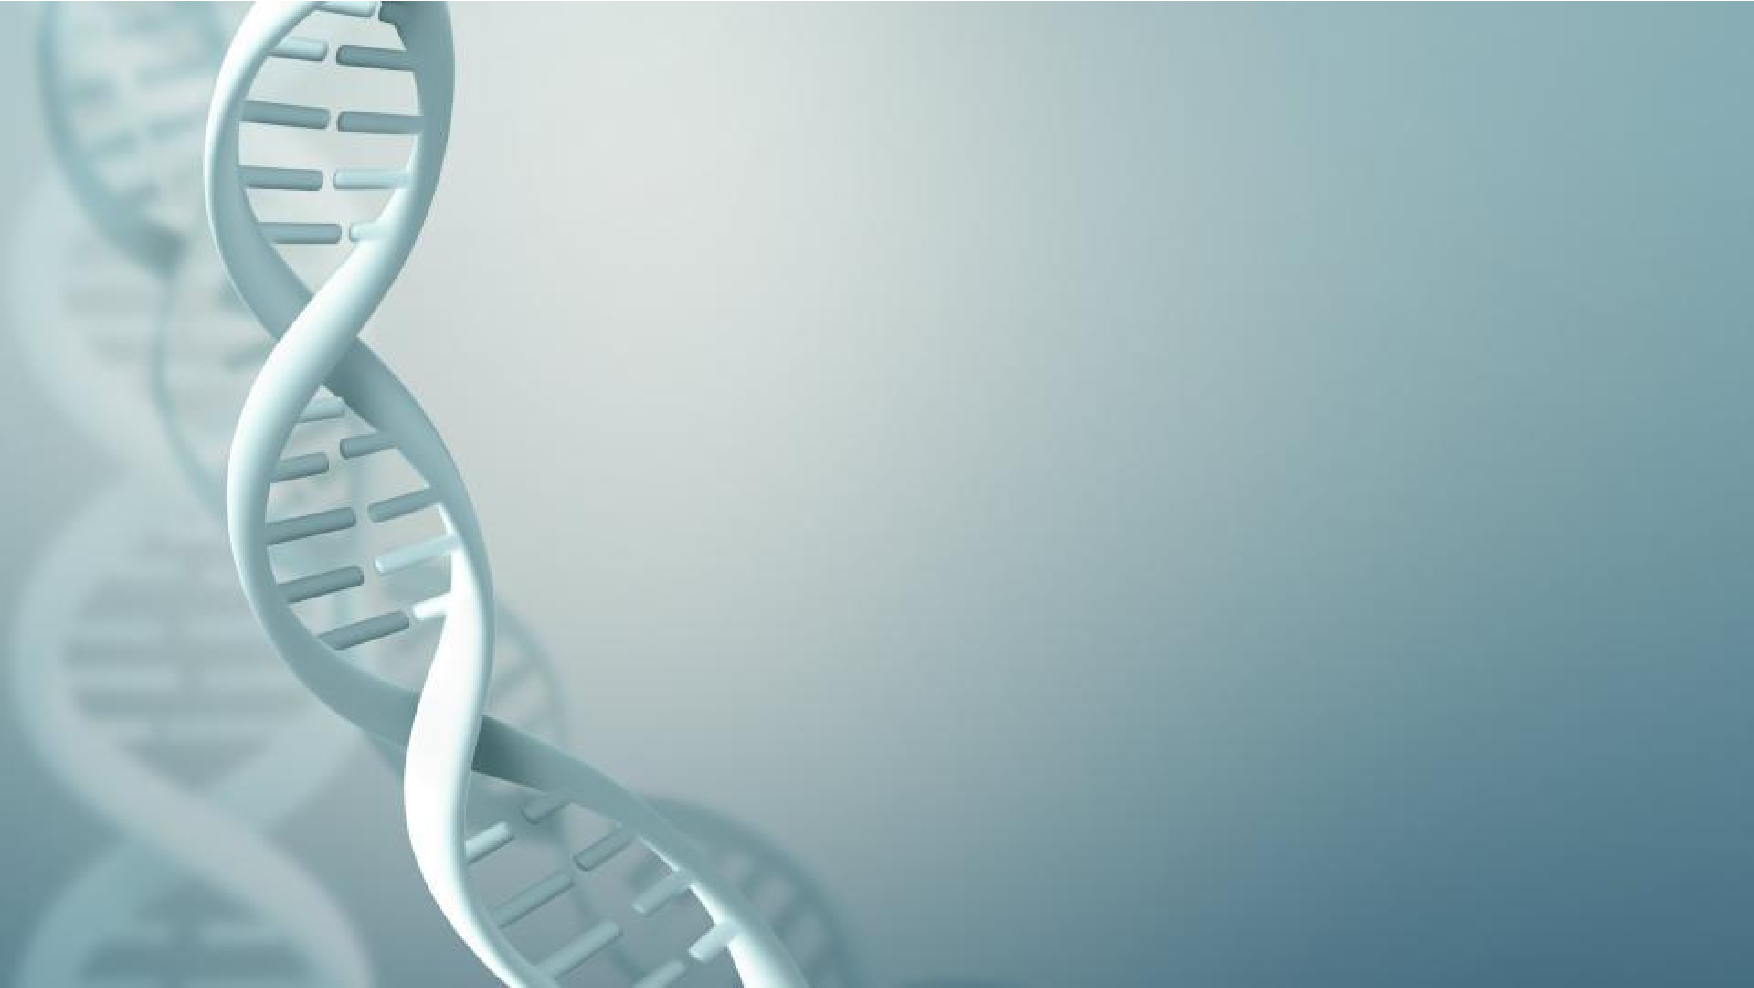
\includegraphics[width=\paperwidth,height=\paperheight]{img/1}
		\tikz[overlay] \fill[fill opacity=0.75,fill=white] (0,0) rectangle (-\paperwidth,\paperheight);
	}
}



%-------------------------------------------------------
% THE BODY OF THE PRESENTATION
%-------------------------------------------------------

\begin{document}
	
	
	\AtBeginSection[]
	{
		\begin{frame}
			\frametitle{Table of Contents}
			\tableofcontents[currentsection]
		\end{frame}
	}
	
	
%-------------------------------------------------------
% THE TITLEPAGE
%-------------------------------------------------------

\if\mycmd1 % MY THEME
\1{
	\begin{frame}[plain,noframenumbering] 
		\titlepage 
	\end{frame}}
	\else % CS THEME
	\maketitle
\fi

%-------------------------------------------------------
%-------------------------------------------------------
\begin{frame}{Table of Contents}
\tableofcontents
\end{frame}
%-------------------------------------------------------
%-------------------------------------------------------


\section{Introduction}

%%%%%%%%%%%%%%%%%%%%%%%%%%%%%%%%%%%%%%%%%%%%%%%%%%%%%%%%
\subsection{Objectives}
%%%%%%%%%%%%%%%%%%%%%%%%%%%%%%%%%%%%%%%%%%%%%%%%%%%%%%%%

%-------------------------------------------------------
%-------------------------------------------------------
\begin{frame}{Objectives}{}
\begin{itemize}
    \item<1-> Understand the size of our genome. 
    \item<2-> Understand the lack of research in Genomics.
  \end{itemize}
\end{frame}
%-------------------------------------------------------
%-------------------------------------------------------

%%%%%%%%%%%%%%%%%%%%%%%%%%%%%%%%%%%%%%%%%%%%%%%%%%%%%%%%
\subsection{The biology of cells: Summary}
%%%%%%%%%%%%%%%%%%%%%%%%%%%%%%%%%%%%%%%%%%%%%%%%%%%%%%%%

%-------------------------------------------------------
%-------------------------------------------------------
\begin{frame}{Introduction}{The biology of cells: Summary}
\begin{figure}[]
 \centering
    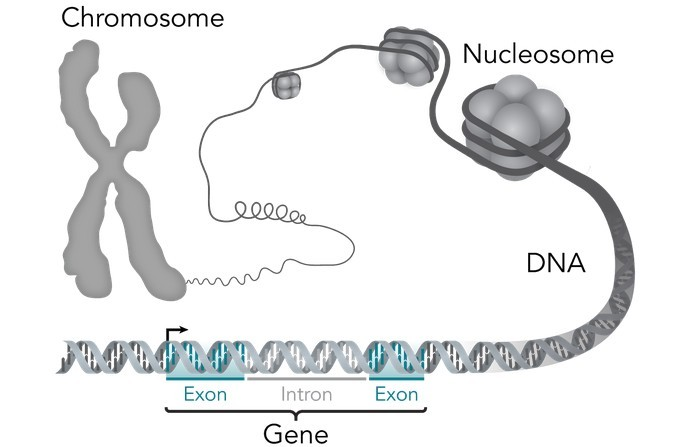
\includegraphics[width=\textwidth,height=0.6\textheight,keepaspectratio]{img/introduction/bio8.jpg}
    \label{img:mot2}
    \caption{Chromosome-DNA-gene \cite{dnacromosome2020}.}
\end{figure}
\end{frame}
%-------------------------------------------------------
%-------------------------------------------------------

%-------------------------------------------------------
%-------------------------------------------------------
\begin{frame}{Introduction}{The biology of cells: Summary}
\begin{figure}[]
 \centering
    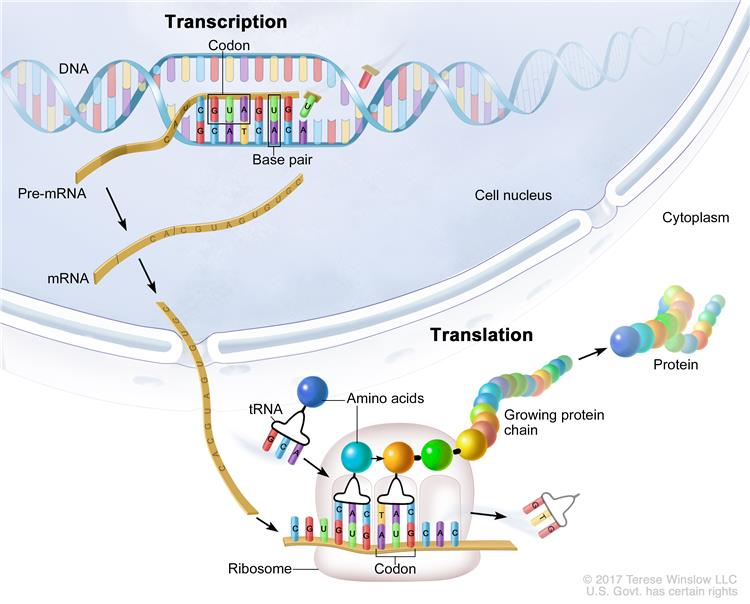
\includegraphics[width=\textwidth,height=0.7\textheight,keepaspectratio]{img/numbers/trans.jpg}
    \label{img:mot2}
    \caption{Transcription and translation \cite{nci2020}.}
\end{figure}
\end{frame}
%-------------------------------------------------------
%-------------------------------------------------------

%-------------------------------------------------------
%-------------------------------------------------------
\begin{frame}{Introduction}{The biology of cells: Summary}
\begin{figure}[]
 \centering
    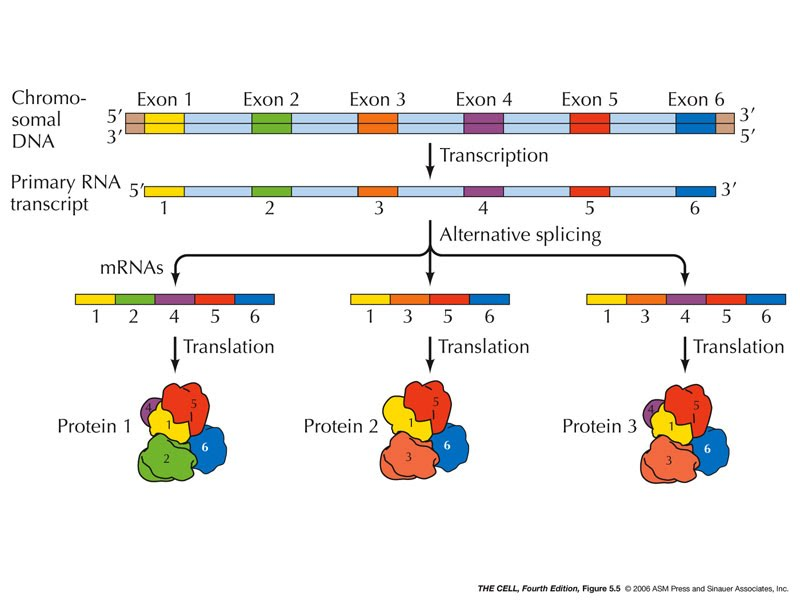
\includegraphics[width=\textwidth,height=0.7\textheight,keepaspectratio]{img/numbers/alt.jpg}
    \label{img:mot2}
    \caption{Alternative splicing \cite{genbio2020}.}
\end{figure}
\end{frame}
%-------------------------------------------------------
%-------------------------------------------------------


\section{Numbers and Databases}

%%%%%%%%%%%%%%%%%%%%%%%%%%%%%%%%%%%%%%%%%%%%%%%%%%%%%%%%
\subsection{Genomes by numbers}
%%%%%%%%%%%%%%%%%%%%%%%%%%%%%%%%%%%%%%%%%%%%%%%%%%%%%%%%

%-------------------------------------------------------
%-------------------------------------------------------
\begin{frame}{Numbers and Databases}{Numbers of base pairs}

\begin{block}{}
\centering
The human genome is made of \textbf{\string ~3.2 billions bp} of DNA. \\
\string ~6.4 billions of nucleotides \cite{archibald2018genomics}.
\end{block}

\begin{block}{}
\centering
The HIV-1 genome is made of \textbf{\string ~20k bp} of DNA. \\
Meanwhile, the COVID-19 is made of \textbf{\string ~32k bp} \cite{randhawa2020machine}.
\end{block}


\end{frame}
%-------------------------------------------------------
%-------------------------------------------------------

%-------------------------------------------------------
%-------------------------------------------------------
\begin{frame}{Numbers and Databases}{Numbers of genes}

\begin{block}{}
\centering
There are approximately \textbf{19000} to \textbf{25000} genes. \\
No one knows for sure \cite{archibald2018genomics}.
\end{block}
\end{frame}
%-------------------------------------------------------
%-------------------------------------------------------

%-------------------------------------------------------
%-------------------------------------------------------
\begin{frame}{Numbers and Databases}{Percentage of protein-coding genes}

\begin{block}{}
\centering
Only \textbf{\string ~1 per cent} of the human genome correspond to protein-coding genes. \cite{archibald2018genomics}.
\end{block}

\begin{block}{}
\centering
Human genes have dozens of introns, each of which can be tens of thousands of nucleotides. Distinguishing exons from introns and other forms of non-coding DNA is challenging \cite{archibald2018genomics}.
\end{block}

\end{frame}
%-------------------------------------------------------
%-------------------------------------------------------

%%%%%%%%%%%%%%%%%%%%%%%%%%%%%%%%%%%%%%%%%%%%%%%%%%%%%%%%
\subsection{Databases}
%%%%%%%%%%%%%%%%%%%%%%%%%%%%%%%%%%%%%%%%%%%%%%%%%%%%%%%%

%-------------------------------------------------------
%-------------------------------------------------------
\begin{frame}{Numbers and Databases}{Databases}

\begin{tabular}{ll}
\textbf{Database} & \textbf{Description}                                                \\
\hline
\href{https://www.ncbi.nlm.nih.gov/genbank/}{GenBank}   & Genetic sequence database                                       \\
\href{https://blast.ncbi.nlm.nih.gov/Blast.cgi}{BLAST}    & Finds regions of similarity between biological sequences    \\
\href{https://www.viprbrc.org/}{ViPR}     & Viral genomes database                                                       \\
\href{https://www.cancer.gov/}{TCGA}     & The Cancer Genome Atlas                                                       \\
 \href{https://dcc.icgc.org/}{ICGC}     & International Cancer Genome Consortium                        \\      
\end{tabular}

\end{frame}
%-------------------------------------------------------
%-------------------------------------------------------


%-------------------------------------------------------
%-------------------------------------------------------
\begin{frame}{Numbers and Databases}{Databases types}
\centering
\begin{tabular}{ll}
\textbf{Primary} & \textbf{Secondary}                                \\
\hline
GenBank    & RefSeq    \\
UniProt    & Genes  \\
PubMed    & Taxon  \\
PMC    & OMIM  \\
Intact & ICGC \\
\end{tabular}

\end{frame}
%-------------------------------------------------------
%-------------------------------------------------------


%-------------------------------------------------------
%-------------------------------------------------------
\begin{frame}{Numbers and Databases}{Databases}
\begin{figure}[]
 \centering
    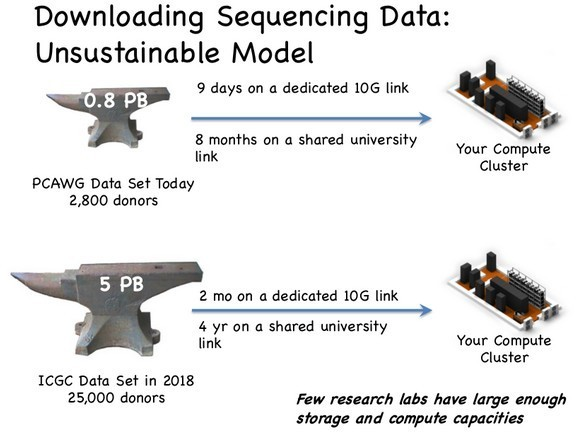
\includegraphics[width=\textwidth,height=0.7\textheight,keepaspectratio]{img/numbers/dat.jpg}
    \label{img:mot2}
    \caption{Downloading sequencing data}
\end{figure}
\end{frame}
%-------------------------------------------------------
%-------------------------------------------------------

%-------------------------------------------------------
%-------------------------------------------------------
\begin{frame}{Numbers and Databases}{Cloud computing and new software paradigm}
\begin{itemize}
\item Data sets are in Petabyte and soon Exabyte scale.
\item Data (and the security rules that come with it) will be somewhere (not in our own data centre), and you will move your software to it.
\end{itemize}
\end{frame}
%-------------------------------------------------------
%-------------------------------------------------------




%%%%%%%%%%%%%%%%%%%%%%%%%%%%%%%%%%%%%%%%%%%%%%%%%%%%%%%%
\subsection{DNA sequence formats}
%%%%%%%%%%%%%%%%%%%%%%%%%%%%%%%%%%%%%%%%%%%%%%%%%%%%%%%%

%-------------------------------------------------------
%-------------------------------------------------------
\begin{frame}{Numbers and Databases}{Cloud computing and new software paradigm}
\begin{itemize}
\item FASTA, FASTAQ.
\item EMBL.
\item GCG.
\item GenBank.
\end{itemize}
\end{frame}
%-------------------------------------------------------
%-------------------------------------------------------



%-------------------------------------------------------
%-------------------------------------------------------
\begin{frame}{Numbers and Databases}{FASTA format}
\begin{figure}[]
 \centering
    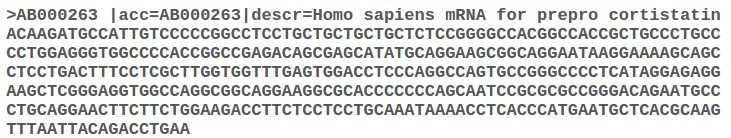
\includegraphics[width=\textwidth,height=0.7\textheight,keepaspectratio]{img/numbers/fasta.jpg}
    \label{img:mot2}
    \caption{FASTA format example}
\end{figure}
\end{frame}
%-------------------------------------------------------
%-------------------------------------------------------

%-------------------------------------------------------
%-------------------------------------------------------
\begin{frame}{Numbers and Databases}{EMBL format}
\begin{figure}[]
 \centering
    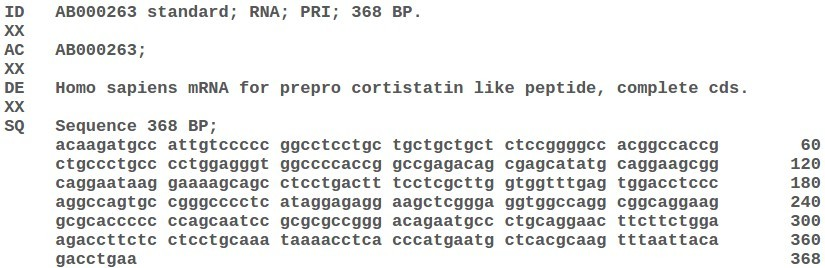
\includegraphics[width=\textwidth,height=0.7\textheight,keepaspectratio]{img/numbers/embl.jpg}
    \label{img:mot2}
    \caption{EMBL format example}
\end{figure}
\end{frame}
%-------------------------------------------------------
%-------------------------------------------------------

%-------------------------------------------------------
%-------------------------------------------------------
\begin{frame}{Numbers and Databases}{A2M format}
The \textbf{A2M format} is used as the primary format for multiple alignments of protein or nucleic-acid sequences. For proteins, the legal alphabet is:
\begin{itemize}
    \item  ACDEFGHIKLMNPQRSTVWY for amino acids
    \item  X for any amino acid
    \item  B for N or D
    \item  Z for Q or E
    \item  O for creating a free-insertion module (FIM) 
\end{itemize}

For nucleic acids, the legal alphabet in SAM is:
\begin{itemize}
    \item  ACGTU for nucleotides (with T and U considered equivalent)
    \item  Y for C or T
    \item  R for A or G
    \item  N for any nucleotide
    \item  O for creating a free-insertion module (FIM) 
\end{itemize}
\end{frame}
%-------------------------------------------------------
%-------------------------------------------------------

%-------------------------------------------------------
%-------------------------------------------------------
\begin{frame}{Numbers and Databases}{GOBLET}
\begin{figure}[]
 \centering
    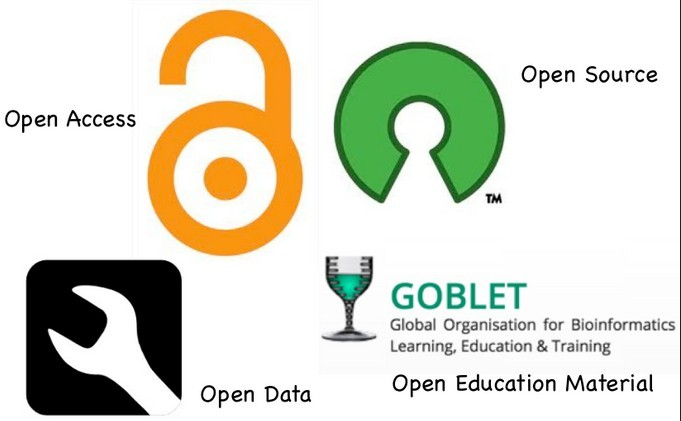
\includegraphics[width=\textwidth,height=0.6\textheight,keepaspectratio]{img/numbers/gob.jpg}
    \label{img:mot2}
    \caption{GOBLET}
\end{figure}
\end{frame}
%-------------------------------------------------------
%-------------------------------------------------------


%-------------------------------------------------------
%-------------------------------------------------------
\begin{frame}{Bioinformatics}{Homework}
	Register to the following courses and bring yours certificated of accomplish: \\
	\begin{itemize} 
		%\item \href{https://edu.t-bio.info/course/introduction-bioinformatics/}{Introduction to Bioinformatics (6 hours) } \\
		\item \href{https://edu.t-bio.info/course/introduction-to-genomics/}{Introduction to Genomics (4 hours)}
	\end{itemize}
\end{frame}
%-------------------------------------------------------
%-------------------------------------------------------


%-------------------------------------------------------
%-------------------------------------------------------
\begin{frame}[allowframebreaks]
        \frametitle{References}
        %\bibliographystyle{amsalpha}
        \bibliographystyle{IEEEtran}
        \bibliography{bibliography.bib}
\end{frame}
%-------------------------------------------------------
%-------------------------------------------------------

%-------------------------------------------------------
%-------------------------------------------------------
\if\mycmd1 % MY THEME
\1{
	{\1
		\begin{frame}[plain,noframenumbering]
			\finalpage{Thank you}
		\end{frame}}
		\else % CS THEME
		
\fi
%-------------------------------------------------------
%-------------------------------------------------------



\end{document}